%	This subsection provides some info on the controllers that run on AtlantikSolar

\begin{figure}[tb]
    \centering
     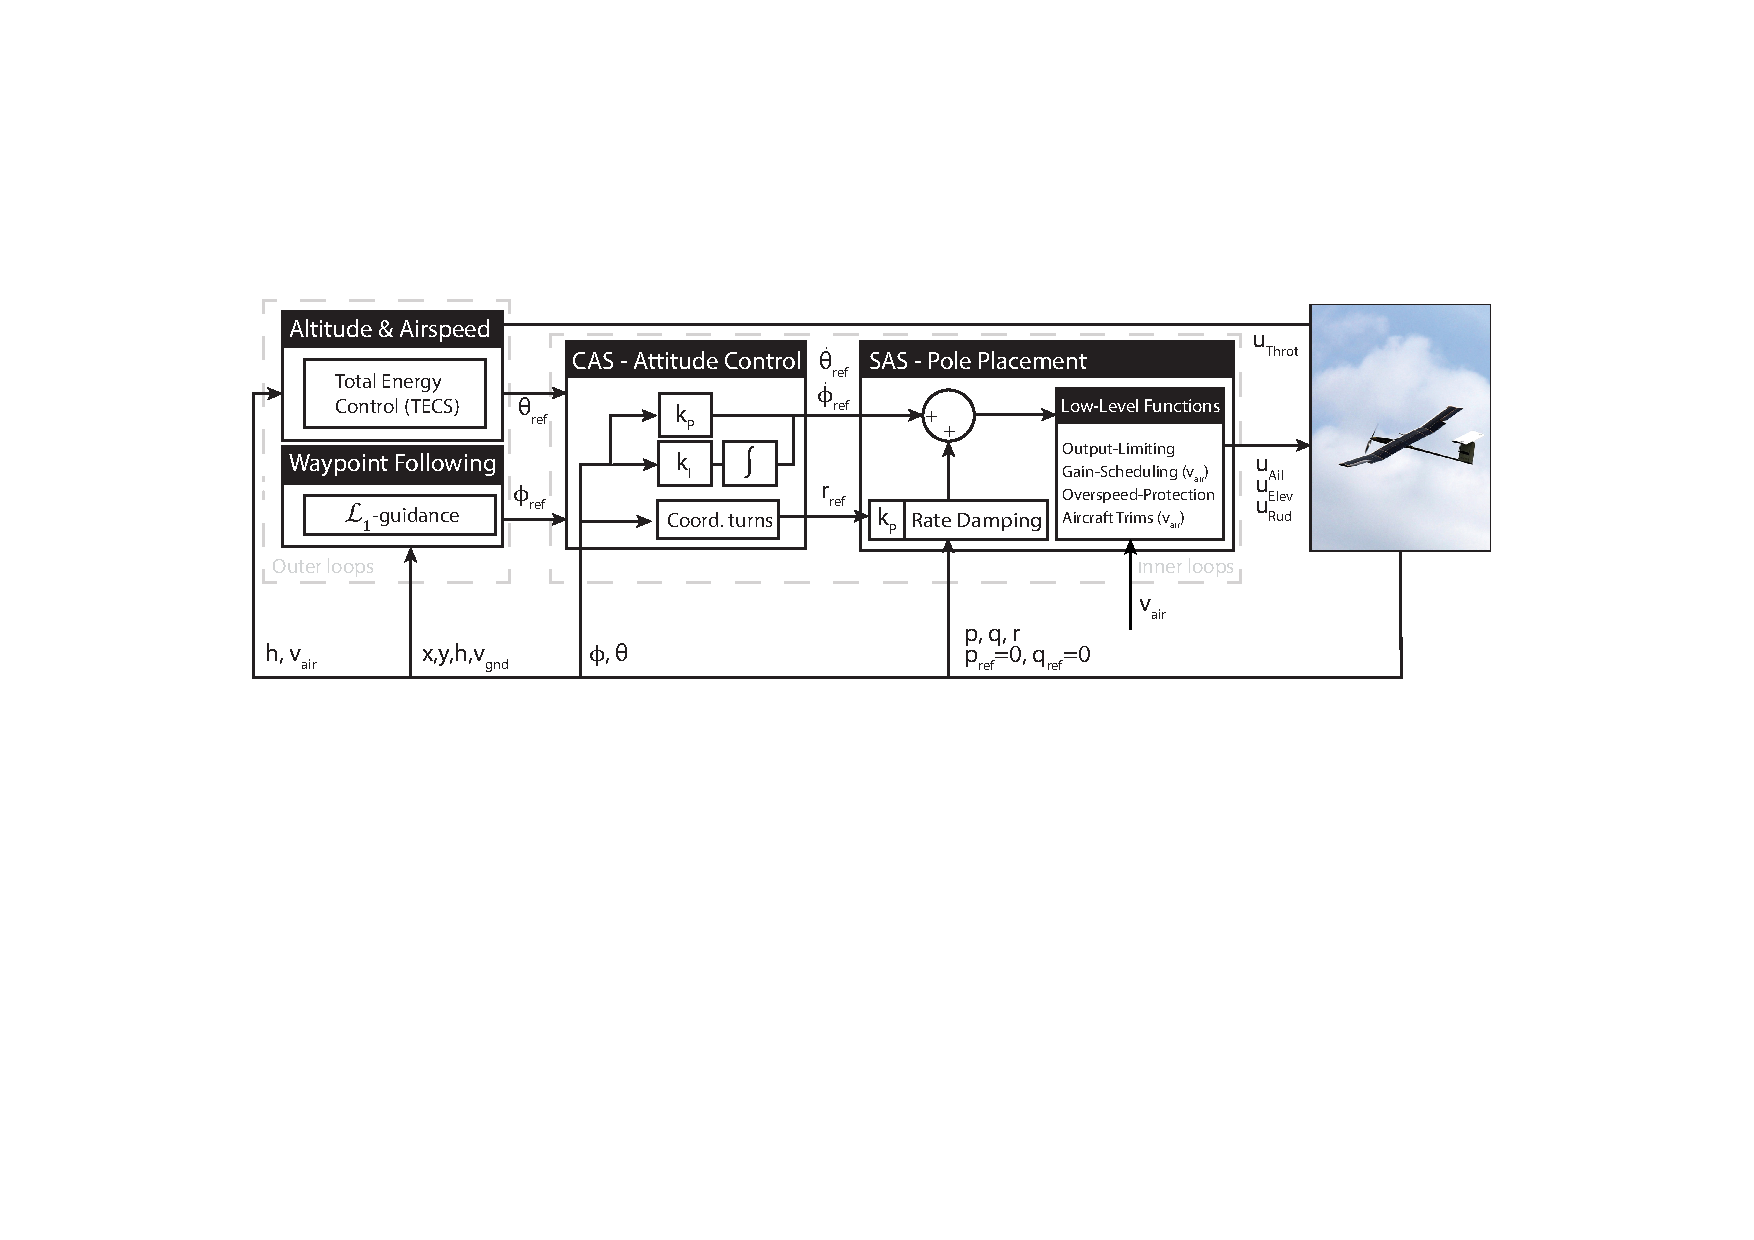
\includegraphics[width=\linewidth]{images/11_ControlScheme/ControlScheme.pdf}
    \caption{Control Scheme implemented for AtlantikSolar.}
    \label{fig:ControlScheme}
\end{figure}

AtlantikSolar features autonomous navigation and loitering through user--defined waypoints. The complete control structure (Figure~\ref{fig:ControlScheme}) is offline-tuned based on the identified system model (Section~\ref{sec:SystemID}), functionality-tested in an X--Plane 10 Hardware--In--the--Loop (HIL) simulation and finally refined in extensive flight tests. For inner--loop control, our baseline--solution corresponds to a set of cascaded saturated PID controllers: The Stability Augmentation System (SAS) applies rate--damping to shape the airplane's frequency response, while the Control Augmentation System (CAS) applies proportional--integral feedback to achieve roll ($\phi$) and pitch ($\theta$) reference tracking. As a cascaded approach, proper tuning requires iteration of the gains to achieve maximum performance and robustness against model uncertainties and external disturbances. Flight tests showed that due to AtlantikSolar's high wingspan and thus high x- and z-axis inertia $I_x$ and $I_z$, coordinated turn control is essential to damp adverse yaw and to achieve the no--sideslip yaw rate $r=\frac{g\cdot \sin(\phi)}{v_{air}}$. To avoid overload of the highly optimized structure, output limiters and an over--speed protection are applied. Furthermore, the control actions are in a final stage adapted with respect to the dynamic pressure $q=\frac{1}{2}\rho v^{2}_{air}$ which accounts for the change of the effective moments created by the control surfaces. 

Once the inner--loops are well--tuned, waypoint guidance is enabled. AtlantikSolar employs a $\mathcal{L}_1$--nonlinear guidance law which generates the lateral acceleration reference $a_{s_{ref}}$ of the UAV based on a look--ahead distance ${L}_1$ and the current velocity $V_T$ and heading error $\eta$ as noted below:

\small
\begin{eqnarray}
 a_{s_{ref}} &=& 2\frac{V_T^2}{L_1}\sin \eta
\end{eqnarray}
\normalsize
which is then kinematically translated to roll references while consistent dynamic behavior is achieved via adaptation of the look--ahead distance as in~\cite{L1stabAnalysis}. This guidance law is integrated into our control structure as described in~\cite{OMLAS_MED_14} and combined with an extended version of the Pixhawk open--source Total Energy Control System (TECS)~\cite{PixhawkWebsite} which provides altitude control: First, a slew rate constraint on the reference altitude $h_{ref}$ has been integrated to reach smoother altitude control at pre-definable climb and sink rates, which is especially important for low propulsion-power to weight-ratio UAVs such as AtlantikSolar. Second, we have implemented \textit{thermal compliance}: In an updraft, the standard TECS implementation will decrease $\theta_{ref}$ to decrease the altitude if $h>h_{ref}$. To allow gaining potential energy from a thermal, we perform gain-scheduling on TECS configuration parameters such that $\theta_{ref}$ is used only for airspeed control and $u_{Throt}$ only for altitude control. When at $h>h_{ref}$, the plane will thus keep $\theta_{ref}=\theta_{ref}(t)$  such that $v(t)=v_{ref}(t)$ and will gradually disable the motor, potentially gaining altitude for strong thermals. Furthermore, altitude limits have been implemented, i.e. full throttle is forced for $h<h_{min}$, at $h>h_{max}$ we gradually allow a pitch-down and thus altitude decrease again, and at $h>h_{max}+50m$ the controller automatically engages the spoilers for maximum descend rate. The inner PID-based pitch- and roll control loops are executed at a sampling period of $T_{SAS,CAS}=0.01s$, while the high-level $\mathcal{L}_1$\&TECS controllers run with $T_{\mathcal{L}_1,TECS}=0.05s$. Given these settings, the full controller requires less than 4\% CPU load, 5KB of RAM and 47KB Flash memory and is thus computationally lightweight when compared to other Pixhawk applications (see~\cite{OMLAS_MED_14}) such as the state estimation. The whole control application is designed to be modular, and more sophisticated approaches like model-predictive control~\cite{OMLAS_MED_14} and robust $H_\infty$--based controllers~\cite{Mosimann_FT} for inner loop control have been implemented and flown on test planes in addition to our cascaded PID baseline-solution. 